\documentclass[a4paper,twoside, openright,12pt]{report}
\usepackage{psfrag,amsbsy,graphics,float}
\usepackage{graphicx, color} %Deleted [dvips] in front of {graphicx, color} for usage also with PDFLaTex
\usepackage[latin1]{inputenc}
\usepackage{verbatim}
\usepackage{tcolorbox}

% based on the LSR Student Template, last change: 2014-06-05

%_______Kopf- und Fußzeile_______________________________________________________
\usepackage{fancyhdr}
\pagestyle{fancy}
%um Kopf- und Fußzeile bei chapter-Seiten zu reaktivieren
\newcommand{\helv}{%
   \fontfamily{phv}\fontseries{a}\fontsize{9}{11}\selectfont}
\fancypagestyle{plain}{
	\fancyfoot{}% keine Fußzeile
	\fancyhead[RE]{\helv\leftmark}% Rechts auf geraden Seiten=innen; in \leftmark stehen \chapters
	\fancyhead[LO]{\helv\rightmark}% Links auf ungeraden Seiten=außen;in \rightmark stehen \sections
	\fancyhead[RO,LE]{\thepage}}%Rechts auf ungeraden und links auf geraden Seiten
%Kopf- und Fußzeile für alle anderen Seiten
\fancyfoot{}
\fancyhead[RE]{\helv\leftmark}
\fancyhead[LO]{\helv\rightmark}%alt:\fancyhead[LO]{\itshape\rightmark}
\fancyhead[RO,LE]{\thepage}
%________________________________________________________________________________


%_Definieren der Ränder und Längen__________
\setlength{\textwidth}{15cm}
\setlength{\textheight}{22cm}
\setlength{\evensidemargin}{-2mm}
\setlength{\oddsidemargin}{11mm}
\setlength{\headwidth}{15cm}
\setlength{\topmargin}{10mm}
\setlength{\parindent}{0pt} % Kein Einrücken beim Absatz!!
%___________________________________________

%_Hyperref for CC Url__________
\usepackage{hyperref}
%___________________________________________

%_______Title Page__________________________________________
\begin{document}
\pagestyle{empty}
\enlargethispage{4.5cm} %Damit das Titelbild weit genug unten ist!
\begin{center}
\phantom{u}
\vspace{0.5cm}
\Huge{\sc Real-time robot arm control using motor imaginary movements decoded from EEG
	signals}\\
\vspace{1.5cm}
		\large{
			RESEARCH PRACTICE\\%i.e. DIPLOMA THESIS, BACHELOR THESIS, ADVANCED SEMINAR,
			%Intermediate Report\\
			\vspace{0.4cm}
			submitted by\\
			Juri Fedjaev\\
			% if this is a diploma/bachelor/master thesis include the following:
			%\vspace{0.5cm}
			%born on: DD.MM.YYYY\\
			%\vspace{0.5cm}
			%Streetname XX \\
			%Zipcode City \\
			%Tel.: xxx\,xxxxxxxx \\
			\vspace{1.5cm}
			NEUROSCIENTIFIC SYSTEM THEORY\\
			Technische Universit\"at M\"unchen\\
			\vspace{0.3cm}
			Prof. Dr J\"org Conradt\\
		}
\end{center}
\vspace{5.5cm}
\begin{tabular}{ll}
Supervisor: &Dipl.-Ing. Zied Tayed \\
% add the start and intermediate report dates for DA/BA/MA thesis
%Start: & xx.xx.201x  \\
%Intermediate Report: &  xx.xx.201x  \\
Final Submission: &  22.05.2017 \\
\end{tabular}
%____________________________________________________________

\newpage	
\cleardoublepage



\phantom{u}
\phantom{1}\vspace{6cm}
\begin{center}
In your final hardback copy, replace this page with the signed exercise sheet.
\end{center}

\newpage


%_______Abstract_____________________________________________
\topmargin5mm
\textheight220mm
\pagenumbering{arabic}
\phantom{u}
\begin{abstract}
  A short (1--3 paragraphs) summary of the work. Should state the problem, major assumptions, basic idea of solution, results. Avoid non--standard terms and acronyms. The abstract must be able to be read completely on its own, detached from any other work (e.g., in collections of paper abstracts). Don't use references in an abstract.
\end{abstract}
%____________________________________________________________

\newpage

%_______Widmung_______________________________________________
\phantom{u}
\phantom{1}\vspace{6cm}
\begin{center}
%Hier die Widmung oder leer lassen
\end{center}
%_____________________________________________________________



\pagestyle{fancy}

%_________Inhaltsverzeichnis__________________________
\tableofcontents	
%_____________________________________________________32



%_________Einleitung__________________________________
\chapter{Introduction}
\begin{itemize}
	\item Introduce the idea of the BCI
	\item applications of BCI for robotic control
	\subitem $\rightarrow$ importance (why robotic arm control), technical difficulties \& limitations, challenges ...
\end{itemize}

\begin{tcolorbox}
\textbf{Problem description:}\\
Brain machine interface (BMI) is used to control a system through which people with motor
disabilities could achieve a better quality of life by improving their interaction ability with the
surrounding environment. Using BMI, patients suffering from severe motor disabilities can also
control robot arm to carry out their activity of daily living by just generating control commands using
their own EEG signals.
\end{tcolorbox}

Your first chapter in the document.
Introduce the problem (gently!). Try to give the reader an appreciation of the difficulty, and an idea of how you will go about it. It's like the overture of an opera: it plays on all the relevant themes.

Make sure you clearly state the vision/aims of your work, what problem you are trying to solve, and why it is important. While the introduction is the part that is read first (ignoring title and abstract) it is usually best written last (when you actually know what you have really achieved). Remember, it's the first thing that is being read, and will have a major influence on the how the reader approaches your work. If you bore them now, you've most likely lost them already. If you make outrageous claims pretend to solve the world's problems, etc, you're likely fighting an uphill battle later on. Also, make sure you pick up any threads spun in the introduction later on, to ensure that the reader thinks they get what they have been promised. Don't create an expectation that you'll deliver more than you actually do. Remember, the reader may be your marker (of a thesis) or referee (of a paper), and you don't want to annoy them.

\section{Problem Statement}
\label{sec:problem}
Excerpt from the description of the practical project: 
\begin{tcolorbox}
The main objective of this project is to implement the algorithm described in \cite{meng2016noninvasive,yong2015eeg} to discriminate and
decode four motor imagery movements (left hand, right hand, both hand imaginary movement and
rest) from EEG signals. Afterwards, the developed algorithm has to be used to control a robot arm in a
real-time scenario.

\textbf{Tasks:}\\
This project requires the student to:
\begin{itemize}
	\item Implement an existing algorithm to classify four motor imaginary movements from EEG
	recorded signals.
	\item Test and validate the developed algorithm in a real-time scenario when the user imagines one
	of the four actions, this imagination would be decoded with a BMI and the robotic arm
	executes the desired movement.
\end{itemize}


\textbf{Optional task:}
\begin{itemize}
	\item Extend the work by using the implemented algorithm to classify reach and grasp imaginary
	movements
\end{itemize}
\end{tcolorbox}

\section{Related Work}
This section will review existing approaches and possible solutions to the problem stated in section~\ref{sec:problem}.
\begin{itemize}
	\item Discuss related projects from other research groups (e.g. TU Graz virtual reality navigation using MI, ...)
	\item past achievements in the area of MI for BCI
	\item provide background information (e.g. motor imagery, motor cortex location and importance for project, local field potentials, ...)
\end{itemize}

%____________________________________________________



%_____Kapitel 2_________________________________
\chapter{Solution Design and Implementation}
Figure below depicts the essential information flow for a BCI system. 
\begin{figure}[htbp]
	\centering
	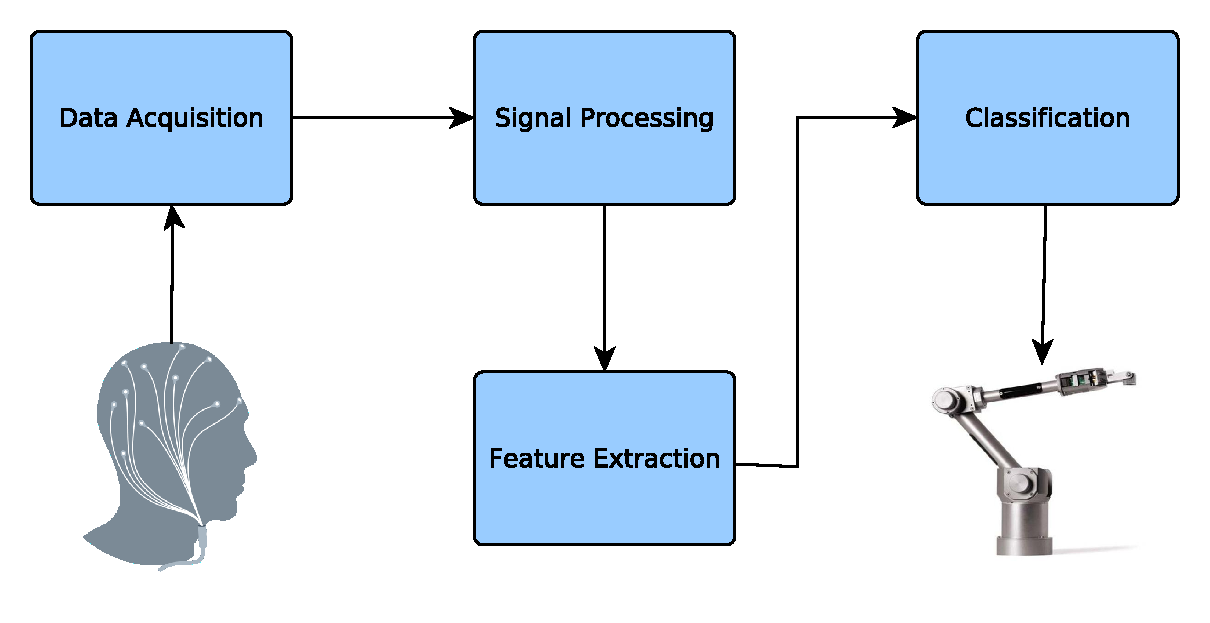
\includegraphics[width=0.9\linewidth]{./gfx/BCI_control_system.pdf}
	\caption{Information flow for a BCI system controlling a robotic arm}
	\label{fig:bci_control_system}
\end{figure}



\section{Experimental Design}
In this section the design of the proposed solution will be described, i.e. the overall architecture on an abstract level. 

\begin{itemize}
	\item OpenVibe
	\item BCILAB
	\item ... 
	\item my Design
\end{itemize}

Experiment design:
\begin{itemize}
	\item cue-based experiment
	\item acquiring samples 
\end{itemize}

In this section, the implementation will be explained in greater detail. 
\begin{itemize}
	\item Chain of information processing
	\item Implementation in Matlab
	\item e
\end{itemize}


\section{Experimental Results}

\begin{itemize}
	\item reached accuracies of SVM
	\item how to ensure that recording is successful  
	\item ...
\end{itemize}


\section{Discussion}
\begin{itemize}
	\item how to improve classification accuracy
	\subitem improve feature extraction, e.g. use ERD / ERS on $\alpha$- / $\beta$-bands 
	\item use different classifier 
	\subitem ANN or SNN would be interesting to see. See paper xy for examples
	\subitem Convolutional NN or recurrent deep NN could significantly improve classification accuracy and therefore enable the system for a multiclass (more than two for instance) classification 
\end{itemize}


Discuss and explain your results. Show how they support your thesis (or, if they don't, give a convincing explanation). It is important to separate objective facts clearly from their discussion (which is bound to contain subjective opinion). If the reader doesn't understand your results, reconsider if you have managed to extract the core information and explain it in a straightforward way.

%_______________________________________________



%_____Zusammenfassung, Ausblick_________________________________
\chapter{Conclusion}

Don't leave it at the discussion: discuss what you/the reader can learn from the results. Draw some real conclusions. Separate discussion/interpretation of the results clearly from the conclusions you draw from them. (So-called "conclusion creep" tends to upset reviewers. It means surrendering your scientific objectivity.) Identify all shortcomings/limitations of your work, and discuss how they could be fixed ("future work"). It is not a sign of weakness of your work, if you clearly analyse and state the limitations. Informed readers will notice them anyway and draw their own conclusions, if not addressed properly.

\vspace{\baselineskip}
Recap: don't stick to this structure at all cost. Also, remember that the thesis must be:

\begin{itemize}
	\item honest, stating clearly all limitations;
	\item self--contained, don't write just for the locals, don't assume that the reader has read the same literature as you, don't let the reader work out the details for themselves.
\end{itemize}



This chapter is followed by the list of figures and the bibliography. If you are using acronyms, listing them (with the expanded full name) before the bibliography is also a good idea. The acronyms package helps with consistency and an automatic listing.


%_______________________________________________________________


%_____Abbildungsverzeichnis_________________________________
\cleardoublepage
\addcontentsline{toc}{chapter}{List of Figures}
\listoffigures 	 %Abbildungsverzeichnis

%___________________________________________________________

%_____Literaturverzeichnis_________________________________
\cleardoublepage
\addcontentsline{toc}{chapter}{Bibliography}
\bibliographystyle{ieeetr}
\bibliography{mybib}

%__________________________________________________________


%_____License_________________________________
\cleardoublepage
\chapter*{License}
\markright{LICENSE}
This work is licensed under the Creative Commons Attribution 3.0 Germany
License. To view a copy of this license,
visit \href{http://creativecommons.org/licenses/by/3.0/de/}{http://creativecommons.org} or send a letter
to Creative Commons, 171 Second Street, Suite 300, San
Francisco, California 94105, USA.
%__________________________________________________________

\end{document}
\grid
